\documentclass{VUMIFPSkursinis}
\usepackage{algorithmicx}
\usepackage{algorithm}
\usepackage{algpseudocode}
\usepackage{amsfonts}
\usepackage{amsmath}
\usepackage{bm}
\usepackage{caption}
\usepackage{color}
\usepackage{float}
\usepackage{graphicx}
\usepackage{listings}
\usepackage{subfig}
\usepackage{url}
\usepackage{wrapfig}
\usepackage[backend=biber]{biblatex}

% Titulinio aprašas
\university{Vilniaus universitetas}
\faculty{Matematikos ir informatikos fakultetas}
\department{Programų sistemų katedra}
\papertype{Kursinis darbas}
\title{Didelių duomenų srautų analizė, anomalijų aptikimas}
\titleineng{Big data analysis, detection of anomalies}
\status{3 kurso 3 grupės studentas}
\author{Jokūbas Rusakevičius}
\supervisor{dr. Vytautas Valaitis}
\date{Vilnius – \the\year}

% Nustatymai
\setmainfont{Palemonas}

\bibliography{bibliografija}

\begin{document}
\maketitle

\tableofcontents

\sectionnonum{Įvadas}
Šis darbas yra Programų Sistemų studijų trečio kurso privalomas kursinis darbas apie anomalijų aptikimą didžiuosiuose duomenyse (angl. \textit{Big Data}) bei anomalijų aptikimą naudojant atviro kodo analitinį įrankį „MacroBase“.

\subsectionnonum{Problematika}
Remiantis 2001 metais „Gartner“ pateiktu apibrėžimu (iki šiol laikomu pagrindiniu (angl. \textit{go-to})), didieji duomenys - tai duomenys, kurie turi didelę įvairovę (angl. \textit{variety}), yra renkami nuolat didėjančiais kiekiais (angl. \textit{volumes}) ir generuojami vis didėjančiais greičiais (angl. \textit{velocity}), šis apibrėžimas dar vadinamas tryjų „V“ \cite{three_vs}. Paprastai, didžiuosius duomenis galima apibrėžti kaip duomenų rinkinius tokius didelius, kad tradiciniai programiniai duomenų apdorojimo įrankiai nesugeba jų sugauti, tvarkyti, organizuoti, apdoroti ar su jais dirbti priimtiname laiko intervale \cite{bigdata_tolerable_time}, jie yra paprasčiausiai per dideli ir per daug sudėtingi. Tačiau šie duomenys turi milžinišką potencialą ir gali būti panaudojami sprendžiant verslo ir kitas problemos, kurių sprendimas iki šiol buvo neįmanomas.\par

Generuojant ir saugant milžiniškus kiekius duomenų, natūraliai, užfiksuojami tokie duomenys, kurie išsiskiria ir yra nebūdingi duomenų rinkiniui. Duomenų vienetai kurie yra nukrypę nuo kitų duomenų rinkinyje yra vadinami anomalijomis. Anomalijų aptikimas yra procesas, kurio metu yra aptinkama ir identifikuojama anomalija arba išskirtis (angl. \textit{outlier}) duomenų rinkinyje \cite{anomaly}. Anomalijos yra retas reiškinys, tačiau jų egzistavimas gali reikšti didelį pavojų taikomajai sistemai ar jos naudotojams. Šio darbo metu bus tiriamas anomalijų aptikimas remiantis iš „Backblaze“ 2018 metų (pirmą ketvirtį) duomenų centruose esančių diskų surinkta informacija \cite{backblaze}.\par
Dėl įvairių priežasčių renkamų, saugomų ir operuojamų duomenų kiekiai nuolatos didėja ir netgi gerokai lenkia žmogaus sugebėjimą juos apdoroti ar analizuoti. Didžiosios socialinių tinklų kompanijos Twitter, Facebook ir LinkedIn 2015-2016 metais pranešė kiekviena atskirai fiksuojanti iki 12 milijonų įvykių per sekundę \cite{twitter, facebook, linkedin}. Taip pat negalima pamiršti vis labiau plintančių ir didelius kiekius duomenų generuojančių automatizuotų duomenų šaltinių („Dalykų Interneto“ (angl. \textit{Internet of Things} arba \textit{IoT})). Be to, tokie palankūs veiksniai kaip kylantis automatizuotų duomenų šaltinių populiarumas, pinganti techninė įranga, išvystyti komunikaciniai tinklai bei mažėjančios duomenų saugojimo kainos paskatino dešimčių milijardų dolerių komercines investicijas šių technologijų vystimui \cite{iot_investments}. Dėl šių ir kitų veiksnių numatoma, kad kiekvienais metais bendras duomenų kiekis išaugs po 40\% \cite{iot}, o iki 2020 metų pranašaujama, kad bendras pasaulinis duomenų kiekis peržengs 40 zetabaitų ($4\times{10}^{22}$ baitų) ribą \cite{future_data_volume}.\par

Didžiųjų duomenų laikomos informacijos paslėpta nauda ir svarba yra visuotinai pripažįstama, tačiau ši informacija nėra lengvai išgaunama. Duomenų peržiūra ir analizė sudaro labai didelį krūvį tiek analitikui, tiek analitiniams įrankiams. Fizinė duomenų peržiūra yra paprasčiausiai neįmanoma, o nuolatos didėjantys duomenų kiekiai vis labiau atskiria dėmesio reikalaujančius duomenis ir ribotą dėmesį turintį analitiką. Net ir aukščiausios kvalifikacijos analitikai praneša panaudojantys vos iki 6\% jų surenkamų duomenų \cite{prioritizing_attention}. Todėl atsiranda iššūkis prioritizuoti žmogaus dėmesį. Nors žmogui yra neįmanoma peržiūrėti visų šių duomenų, tačiau kompiuteriai ir/ar mašinos gali. Informacinės sistemos labiau nei bet kada turi filtruoti, akcentuoti, jungti, grupuoti pateiktus duomenis, jiems suteikti kontekstą ir rodyti naudotojui tik ribotą, svarbią bei apibendrintą informaciją. Visa rodoma, bet nereikalinga informacija reikalauja ir eikvoja žmogaus dėmesį \cite{attention}.\par

Standfordo universitetas kartu su Masačusetso technologijos institutu 2017 metais paskelbė kuriantys naują atviro kodo, ne tik didžiųjų, bet ir greitųjų duomenų (angl. \textit{Fast Data}) analitinį paieškos įrankį. „MacroBase“ pagrindinis uždavinys yra žmogaus dėmesio prioritizavimas. Vienas iš „MacroBase“ šio uždavinį sprendimų yra sugeneruoti didžiausio dėmesio reikalaujančią supaprastintą išvestį, kurios neįprastus duomenų vienetus „MacroBase“ padeda aiškinti pagal duomenų atributus \cite{macrobase_overview, prioritizing_attention}. „MacroBase“ yra naujas ir modernus analitinis įrankis, pateikiantis inovatoriškų sprendimų vis didėjančių ir greitėjančių duomenų srautų analizei atlikti bei galintis grąžinti tikslius rezultatus dirbdamas 2 milijonų įvykių per sekundę greičiu per užklausą per branduolį, dėl to, šiame darbe bus plačiau nagrinėjamas bei eksperimentai atliekami naudojant būtent šį įrankį.

\subsectionnonum{Darbo tikslas ir uždaviniai}
Šio darbo \textbf{tikslas} - palyginti iki šiol naudotas didelių duomenų analizavimo technologijas ir pasinaudoti „MacroBase“ duomenų analizavimo ir anomalijų aptikimo įrankį anomalijų aptikimui.\par

Darbui iškelti \textbf{uždavyniai}:\par

\begin{enumerate}
\item Paaiškinti kas yra „Didieji Duomenis“.
\item Surasti ir palyginti dabar naudojamus anomalijų dideliuose duomenyse aptikimo įrankius.
\item Išanalizuoti „MacroBase“.
\item Paruošti eksperimentui reikalingą įrašų rinkinį iš „Backblaze“ kiekvieną ketvirtį skelbiamų duomenų.
\item Įsidiegti ir paruošti darbui „MacroBase“ analitinį įrankį.
\item Atlikti eksperimentus ir aptikti anomalijas paruoštuose duomenyse.
\item Pateikti galutines eksperimento išvadas.
\end{enumerate}

\section{Didieji duomenys}
Pasak MIT Media Lab direktoriaus Joi Ito, duomenų užrašymas ant popieriaus lapo dar visai neseniai buvo vienintelis būdas rinkti informaciją. Žmogus sugalvotas idėjas ir mintis užrašydamas ant popieriaus lapo jas paversdavo žiniomis. Tačiau dabartinė didžiųjų duomenų situacija yra kitokia. Priešingai nei seniau, surenkamų duomenų kiekiai yra milžiniški, tačiau jie nėra žinios, tol kol jų nepradedama nagrinėti ir analizuoti. Tik pradėjus analizuoti duomenis atliekant su jais įvairias transformacijas, galima pastebėti, kad gaunama įdomi ir netgi svarbi informacija\cite{documentary}. \par

Terminas „Didieji duomenys“ vartojamas apibūdinant procesą naudojamą, kai tradicinės duomenų rinkimo (angl. \textit{data mining}) ir tvarkymo metodikos nebegali įžvelgti ar atskleisti duomenyse esančios prasmės \cite{bigdata}. Nors pirmieji dideli duomenų įrašų rinkiniai yra datuojami jau 1960-1970 metais \cite{first_bigdata}, pats terminas buvo pradėtas naudoti tik nuo 1990 metų, o jo autoriumi yra laikomas ar bent už termino išgarsinimą yra dėkojama John Mashley \cite{john_1, john_2, john_3}. Tačiau kaip didžiųjų duomenų „dydis“ nuolatos plečiasi ir kinta, taip ir jų apibrėžimas, bei apibrėžimui naudojamų „V“ kiekis (\ref{subsec:požymiai} poskyris).\par

Didieji duomenys apima visų trijų struktūrizacijos lygių duomenis: struktūrizuotus, iš dalies struktūrizuotus ir nestruktūrizuotus, tačiau dižiausias didžiųjų duomenų dėmesys yra skiriamas nestruktūrizuotiems duomenims \cite{bigdata_data_struct}. Šie skirtingo struktūrizacijos lygio duomenys pasižymi tokiomis savybėmis:

\begin{itemize}
\item \textbf{Struktūrizuoti duomenys} - tai duomenys, laikomi jiems skirtuose fiksuotuose laukuose, failuose ar įrašuose. Struktūrizuoti duomenys priklauso nuo jiems priskirto duomenų modelio, kuris nurodo kokie, kokio tipo (skaitiniai duomenys, valiutos, alfabetiniai duomenys, vardai, datos, adresai) ir kokių apribojimų (simbolių skaičius, terminų apribojimas, pvz.: Ponas, Ponia, Prof., Doc. ir kt) laukai bus saugomi. Šio tipo duomenys yra lengvai operuojami, pridedami ir analizuojami. Dėl didelių duomenų saugojimo kaštų tai  ilga laiką buvo vienintelis sprendimas duomenų saugojimui - viskas, ko negalima optimaliais struktūrizuoti, laikoma popieriniame formate \cite{structured_data}.

\item \textbf{Iš dalies struktūrizuoti duomenys} \cite{semistructured_data} - tai tarpinis variantas tarp struktūrizuotų ir nestruktūrizuotų duomenų. Duomenys neturi jiems priskirtos formalios duomenų modelio struktūros susietos su duomenų bazėmis ar kitomis duomenų lentelių formomis, tačiau turi žymes ar kitas žymėjimo priemones įrašų atskyrimui ir įrašų hierarchijos sukūrimui. Todėl iš dalies struktūrizuoti duomenys yra dar žinomi kaip save apibūdinančios (angl. \textit{self-describing}) struktūros. Iš dalies struktūrizuotuose duomenyse įrašai gali priklausyti vienai klasei ir būti grupuojami kartu, tačiau turėti skirtingus atributus, o pati atributų išdėstymo tvarka nėra svarbi. XML ir kitos žymių kalbos yra iš dalies struktūrizuotų duomenų pavyzdžiai \cite{structured_data}.

\item \textbf{Nestruktūrizuoti duomenys} - tai duomenys, kuriems skiriamas didžiausias didžiųjų duomenų dėmesys. Šio tipo duomenys neturi jiems priskirto duomenų modelio ar taisyklių pagal, kurias jie būtų organizuojami, ir jų neišeina klasifikuoti pagal žmogui skaitomus požymius. Tai daugiaprasmiai duomenys, kurių sudėti tvarkingai į vieną „dėžutę“ yra neįmanoma: nuotraukos, paveikslėliai, vaizdo įrašai, transliuojami instrumentiniai duomenys, PDF dokumentai, pristatymų skaidrės, elektroniniai laiškai, tinklaraščiai, teksto dokumentai, knygos, medicinos įrašai ir kt. Nors kiekvienas prieš tai išvardytas duomenų tipas atskirai yra struktūrizuotas, tačiau jų rinkinys vis tiek laikomas nestruktūrizuotais duomenimis \cite{structured_data}. Yra apskaičiuota, kad apie 80\% visų duomenų yra nestruktūrizuoti \cite{unstructured}.
\end{itemize} 

Toliau šiame skyriuje bus aprašomi didžiuosius duomenis apibūdinantys penki „V“ (\ref{subsec:požymiai} poskyris. Galiausiai bus rašoma apie didžiųjų duomenų pritaikymą (\ref{subsec:pritaikymas} poskyris).

\subsection{Didžiųjų duomenų didieji „V“} \label{subsec:požymiai}
Originaliai 2001 metais pateiktas didžiųjų duomenų apibrėžimas susidėjo iš trijų „V“: įvairovės (angl. \textit{variety}), kiekio (angl. \textit{volume}) ir greičio (angl. \textit{velocity}) \cite{three_vs}. Tačiau per paskutinius kelis metus šis apibrėžimas buvo papildytas dviem naujais „V“: duomenų teisingumu (angl. \textit{veracity}) ir verte (angl. \textit{value}) \cite{five_vs_everyone_must_know}. 2016 metais pateiktas atnaujintas didžiųjų duomenų apibrėžimas: didžiuosius duomenis sudaro informacijos rinkiniai charakterizuojami tokių aukštų duomenų kiekių, greičių ir įvairovės, kad yra reikalingos specifinės technologijos ir analitiniai metodai vertės iš tos informacijos išgavimui \cite{bigdata_16}. Toliau šiame poskyryje bus aprašomas kiekvienas „V“ (Kiekis (\ref{subsubsec:kiekis} punktas), greitis (\ref{subsubsec:greitis} punktas), įvarovė (\ref{subsubsec:įvairovė} punktas), teisingumas (\ref{subsubsec:teisingumas} punktas) ir vertė (\ref{subsubsec:vertė} punktas)) atskirai.

\subsubsection{Keikis - „Volume“} \label{subsubsec:kiekis}
\textbf{Kiekis} nusako didžiulį kiekį duomenų, kurie yra sugeneruojami kiekvieną sekundę. „FaceBook“ kiekvieną dieną sugeneruoja 4 petabaitus ($1 PB = {10}^{15} B$) naujų duomenų, vien mygtukas „Patinka“ yra paspaudžiamas virš 4 milijonų kartų per minutę, o naujų kiekvieną dieną įkeliamų nuotraukų skaičius siekia net 350 milijonų \cite{facebook_stats}. Sugeneruojamų duomenų kiekis per minutę beveik prilygsta visiems iki 2008 metų surinktiems duomenims. Tačiau pasinaudojus didžiųjų duomenų technologija ir išskirstytą (angl. \textit{distributed}) sistemą, kur duomenų dalys sujungtos programinės įrangos yra laikomos skirtingose vietose, yra įmanoma juos saugoti ir jais naudotis.

\subsubsection{Greitis - „Velocity“} \label{subsubsec:greitis}
\textbf{Gretis} nusako greitį, kuriuo yra generuojami nauji duomenys, ir greitį kuriuo duomenys yra perduodami. „CERN“ „LHC“ dalelių greitintuvas generuoja 1 megabaitą neapdorotų duomenų per įvykį, o per vieną sekundę yra užregistruojami net 600 milijonų įvykių (iš viso 600 TB/s) \cite{cern}. Didžiųjų duomenų technologijos sudaro sąlygas analizuoti duomenis, kol jie yra generuojami taip niekada nepatalpinant jų į duomenų bazę.

\subsubsection{Įvairovė - „Variety“} \label{subsubsec:įvairovė}
\textbf{Įvairovė} nusako skirtingus duomenų tipus. Dauguma duomenų dabar, ne taip kaip praeityje, yra nestruktūrizuoti, kas padaro juos sunkiai patalpinamus į duomenų lenteles. Pasinaudojus didžiųjų duomenų technologija galima sujungti skirtingų rūšių duomenis kartu su tradiciniais struktūrizuotais duomenimis.

\subsubsection{Teisingumas - „Veracity“} \label{subsubsec:teisingumas}
\textbf{Teisingumas} nusako duomenų netvarkingumą ir patikimumą. Dėl skirtingų didžiųjų duomenų formų, kokybė ir tikslumas yra beveik nevaldomi. Tačiau didieji duomenys ir analitinės technologijos sugeba dirbti su šio tipo duomenimis, dažnai kompensuodamos duomenų netikslumą ir nekokybiškumą dideliais duomenų kiekis.

\subsubsection{Vertė - „Value“} \label{subsubsec:vertė}
\textbf{Vertė} nusako iš didžiųjų duomenų gaunamą naudą ir dažnai yra laikomas svarbiausiu iš visų „V“. Yra svarbu dirbant su didžiaisiais duomenimis paversti juos į tam tikra vertę. Tai nebuvo vienas iš originaliai apibrėžtų „V“, tačiau buvo įvardintas dėl didelių darbo su didžiaisiais duomenimis kaštų ir nevisada aiškios gaunamos naudos.

\subsection{Pritaikymas} \label{subsec:pritaikymas}
Didžiuosius duomenis pritaikymas yra galimas beveik bet kokioje srityje, kur yra generuojami dideli kiekiai duomenų. Didžiųjų duomenų industrija tokia didelė, kad 2010 metais ji buvo verta apie 100 milijardų dolerių ir augo po beveik 10\% per metus \cite{bigdata_industry}. Didieji duomenys yra populiarūs, nes iš jų gaunamos žinos yra plačiai pritaikomos. Todėl didžiųjų duomenų pritaikymo pavyzdžių šiais laikais galima rasti visur:
\begin{itemize}
\item Gamintojai gauna vieną didžiausių naudų. Naudojant didžiuosius duomenis gamintojai gali tobulindami savo tiekimo planus, gaminti pagal numatytą paklausą ir pasiekti beveik nulinį tiekimo laiką.
\item Medicina didieji duomenys yra naudojami siekiant pritaikyti suasmenintą mediciną \cite{in_medicine}.
\item Edukacinės institucijos kaip universitetai pradėjo kurti su duomenų analize susijusias studijų programas 2011 metais paskelbtai 1,5 milijonų aukštos kvalifikacijos duomenų analitikų trūkumo \cite{shortage} paklausai patenkinti.
\item Žiniasklaida naudoja naudoja didžiųjų duomenų analizę pateikdamos suasmenintas, kryptingas reklamas.
\item Kt.
\end{itemize}
Su vis didėjančiais duomenų kiekiais ir generavimo greičiais didėja ir duomenyse esančių žinių potencialas. Remiantis 2014 metų duomenimis, vienas trečdalis visų duomenų yra saugomi skaitiniu ir/ar raidiniu (angl. \textit{alphanumeric}) tekstų arba nuotraukų pavidalu \cite{one_third}, o tai formatas naudingiausias duomenų pritaikymui. Taip pat, didelis potencialas slypi didžiųjų duomenų analizėm nenaudojamuose vaizdo ir audio bei kituose duomenyse.

\section{Didžiųjų duomenų analizavimas}


\section{„MacroBase“ analitinis įrankis}


\section{Duomenų analizės eksperimentas naudojant „MacroBase“ analitinį įrankį}
Eksperimentui atlikti buvo pasirinktas „MacroBase GUI“ analitinio įrankio „MacroBase“ grafinė naudotojo sąsaja. CSV tipo failai buvo pasirinktas duomenų šaltinio tipas atliekant eksperimentą.

\subsection{Duomenų rinkinys}
Šiame poskyryje aprašyti eksperimentui pritaikyti „Backblaze“ standžiųjų diskų stebėjimo duomenys \cite{backblaze}.

\subsubsection{Eksperimentui pritaikyti duomenys}
Eksperimentui bus naudojami „Backblaze“ duomenų centruose esančių standžiųjų diskų atliekamo darbo stebėjimų duomenys. „Backblaze“ nuo 2013 metų kiekvieną ketvirtį paviešina surinktus duomenis stebint jų duomenų centruose esančius kietuosius diskus. Kiekvieno ketvirčio duomenys yra pateikiami CSV failais - vienas CSV failas vienai dienai. Vidutinis vienos dienos įrašų eilučių skaičius faile - 100 tūkst; dydis - 28MB. Eksperimentui buvo pasirinktas, paskutinis paviešintas, 2018 metų pirmo ketvirčio duomenų rinkinys \cite{backblaze} - 90 CSV failų.

\subsubsubsection{Duomenų aprašymas}
Kiekvienas „Backblaze“ duomenų centrų dienos įrašų CSV failas yra sudarytas iš duomenų, kurių didžiąją dalį sudaro „S.M.A.R.T.“ \cite{smart_meaning}, „Save Stebinčios Analizuojančios ir Protokoluojančios Technologijos“ (angl. \textit{„Self-Monitoring, Analysis and Reporting Technology“} dažniausiai sutrumpintai vadinami „SMART“), laukai:

\begin{itemize}
\item \textit{\textbf{Date}} - įrašo įrašymo data, užrašoma yyyy-mm-dd formatu (dėl grupavimo į failus pagal dienas, visi įrašai viename faile turės tą pačią datą).
\item \textit{\textbf{Serial Number}} - gamintojo priskirtas kietojo disko serijos numeris.
\item \textit{\textbf{Model}} - gamintojo priskirtas kietojo disko modelio numeris.
\item \textit{\textbf{Capacity Bytes}} - disko dydis baitais.
\item \textit{\textbf{Failure}} - įvykusios klaidos žymėjimui skirtas laukas. „0“, jei kietasis diskas dirba korektiškai; „1“, jei tai buvo paskutinė diena, kai diskas buvo naudojamas prieš sugesdamas.
\item \textit{\textbf{SMART}} laukai - 100 stulpelių duomenų iš kurių 50 yra neapdorotų ir 50 normalizuotų duomenų stulpelių (laukų reikšmės yra aprašytos prieduose (Priedas \ref{sec:smart})).
\end{itemize}

\subsubsubsection{Duomenų paruošimas}
Eksperimentui atliktas naudojant individualius dienų failus, tačiau dėl didesnio duomenų kiekio faile bei bendros analizės buvo paruošti 4 papildomi CSV failai: kiekvienam mėnesiui po vieną ir viso ketvirčio bendras. Tam buvo parašytas „Bash Shell“ skriptas, kuriam per argumentą yra pateikiama „Backblaze“ CSV failų direktorija. Skriptas pavadintas „combine\_csv.sh“; skriptas grąžina failus pavadinimais: „combine\_all.csv“, „combine\_01.csv“ (sausio mėnesiui), „combine\_02.csv“ (vasario mėnesiui), „combine\_03.csv“ (kovo mėnesiui). Skriptas yra pateiktas prieduose (Priedas \ref{sec:skriptas}).
\begin{itemize}
\item Bendras CSV failas \textbf{„combine\_all.csv“}:
\begin{itemize}
\item Dydis: \textbf{2,5GB};
\item Įrašų eilučių skaičius: \textbf{8 949 492};
\end{itemize}

\item Sausio mėnesio CSV failas \textbf{„combine\_01.csv“}:
\begin{itemize}
\item Dydis: \textbf{846MB};
\item Įrašų eilučių skaičius: \textbf{3 039 306};
\end{itemize}

\item Vasario mėnesio CSV failas \textbf{„combine\_02.csv“}:
\begin{itemize}
\item Dydis: \textbf{782,3MB};
\item Įrašų eilučių skaičius: \textbf{2 803 852};
\end{itemize}

\item Kovo mėnesio CSV failas \textbf{„combine\_03.csv“}:
\begin{itemize}
\item Dydis: \textbf{868,2MB};
\item Įrašų eilučių skaičius: \textbf{3 106 334}.
\end{itemize}
\end{itemize}

\subsection{Eksperimentui naudotos aplinkos aprašimas}
Eksperimentas buvo atliekamas naudojant „Ubuntu (64-bit)“ operacinę sistemą įdiegtą virtualioje mašinoje „Oracle VM VirtualBox“. „MacroBase“ įdiegtas ir paruoštas darbui naudojantis „MacroBase“ dokumentaciją.

\subsubsection{Virtuali mašina eksperimentui}
„MacroBase“ pateikiami pavyzdžiai ir konfigūraciniai nurodymai yra pateikiami „Linux“ operacinėms sistemoms. Todėl eksperimentui atlikti buvo pasirinkta atviro kodo nemokama operacinė sistema „Ubuntu“. Dėl paprastumo buvo nuspręsta operacinei sistemai naudoti virtualią mašiną. Atviro kodo nemokama virtuali mašina „Oracle VM VirtualBox“ buvo pasirinkta šiai užduočiai. Galutinės eksperimentui naudotos sisteminės specifikacijos:
\begin{itemize}
\item „Ubuntu“ operacinės sistemos 64 bitų versija \textbf{„Ubuntu (64-bit)“}, versija: \textbf{16.04 LTS};
\item \textbf{„Oracle VM VirtualBox“}, versija: \textbf{5.2.12} r122591 (Qt5.6.2);
\item Virtualus standusis diskas: \textbf{40GB};
\item Virtualiai mašinai skirta operatyvioji atmintis: \textbf{4GB}.

\end{itemize}

\subsubsubsection{Virtualios mašinos paruošimas}
Virtualios mašinos paruošimas darbui:
\begin{enumerate}
\item  Iš „Oracle VM VirtualBox“ internetinės svetainės atsisiunčiamas naujausias „Windows 10“ (operacinė sistema į kuria diegiama virtuali mašina) operacinę sistemą palaikantis diegimo failas (\url{https://www.virtualbox.org/wiki/Downloads}).
\item Sekant sąrankos vedlio nurodymus įdiegiama „Oracle VM VirtualBox“ virtuali mašina.
\item Iš „Ubuntu“ internetinės svetainės atsisiunčiamas naujausios „Ubuntu (64-bit)“ operacinės sistemos ISO failas (\url{https://www.ubuntu.com/download/desktop}).
\item Atidarius „Oracle VM VirtualBox“ programinę įrangą pradedamas naujos operacinės sistemos pridėjimas spaudžiant ant mygtuko su tekstu „Nauja“.
\item Toliau rodomuose languose: pasirenkamas operacinės sistemos tipas - „Linux“; versija: „Ubuntu (64-bit)“; nurodomas operatyviosios atminties kiekis megabaitais: 4096MB; sukuriamas virtualus standusis diskas: 40GB.
\item „Oracle VM VirtualBox“ pagrindiniame lange pasirinkus naujai sukurtą virtualią mašiną spaudžiama ant mygtuko su tekstu „Paleisti“.
\item Atsiradusiame virtualios mašinos lange pasirenkamas prieš tai atsiųstas „Ubuntu (64-bit)“ ISO failas.
\item Pasirenkama „Install“ ir sekant diegimo vedlį, įdiegiama „Ubuntu (64-bit)“ operacinė sistema.
\end{enumerate}

\subsubsection{„MacroBase GUI“ analitinio įrankio su grafine naudotojo sąsaja paruošimas}
Sekant „MacroBase“ dokumentacijoje nurodytus žingsnius įdiegiamas „MacroBase GUI“ \cite{macrobase_doc}:
\begin{enumerate}
\item Atidaromas „Ubuntu“ Terminalas;
\item Klonuojama projekto repozitorija:\\\code{git clone https://github.com/stanford-futuredata/macrobase.git}
\item Sukompiliuojamas „MacroBase“ ir paruošiamas darbui:\\\code{cd macrobase; mvn package}
\item Paleidžiamas „MacroBase“ serveris su grafinė sąsaja:\\\code{bin/frontend.sh}
\item Atidarius interneto naršyklę „MacroBase GUI“ pasiekiamas adresu: \\\url{http://localhost:8080}
\end{enumerate}
Dirbant su CSV failas tai yra žingsniai, kurių užtenka parengti „MacroBase GUI“ darbui (Priedas \ref{sec:gui}, pav. \ref{img:gui} ir \ref{img:gui2}).

\subsubsubsection{„MacroBase GUI“ reikalingi papildomi paketai}
Diegiant „MacroBase“ į naują „Ubuntu“ operacinę sistemą, reikia įdiegti atitinkamus paketus. Visos reikalingos papildomos „Ubuntu“ terminalo komandos:
\begin{enumerate}
\item Versijavimo kontrolės sistemos „Git“ \cite{git} diegimas:\\\code{sudo apt install git}
\item Java projektų valdymo ir diegimo priemonės „Maven“ \cite{maven} diegimas:\\\code{sudo apt install maven}
\item Java JRE \cite{jre_jdk} diegimas:\\\code{sudo apt-get install default-jre}
\item Java JDK \cite{jre_jdk} diegimas:\\\code{sudo apt-get install default-jdk}
\end{enumerate}

\subsection{Eksperimento vykdymo eiga}
Šiame poskyryje aprašoma eksperimento vykdymo eiga naudojant „Backblaze“ pateiktus 2018 metų pirmo ketvirčio duomenų rinkinius. 
\subsubsection{Eksperimento}


\sectionnonum{Rezultatai ir išvados}
Rezultatų ir išvadų dalyje turi būti aiškiai išdėstomi pagrindiniai darbo
rezultatai (kažkas išanalizuota, kažkas sukurta, kažkas įdiegta) ir pateikiamos
išvados (daromi nagrinėtų problemų sprendimo metodų palyginimai, teikiamos
rekomendacijos, akcentuojamos naujovės).

\printbibliography[heading=bibintoc]

% \sectionnonum{Sąvokų apibrėžimai}
\sectionnonum{Santrumpos}
\begin{itemize}

\end{itemize}
\textbf{CSV} - „Failo formatas, sudarytas iš Kableliais atskirtų reikšmių“ angl. \textit{Comma-Separated Values}.\par

\appendix

\section{„Backblaze“ duomenų S.M.A.R.T. laukų paskirtys} \label{sec:smart}
„Backblaze“ naudoja „S.M.A.R.T.“ technologija kietųjų diskų protokolavimui. Tačiau „Backblaze“ naudoja ne visus „S.M.A.R.T.“ laukų:
\begin{itemize}
\item \textit{\textbf{Smart 1 raw, Smart 1 normalized}} - (nuo gamintojo priklausanti reikšmė) nuskaitymo klaidų dažnis (mažesnis geresnis).
\item \textit{\textbf{Smart 2 raw, Smart 2 normalized}} - bendras disko pralaidumo efektyvumas (didesnis geresnis).
\item \textit{\textbf{Smart 3 raw, Smart 3 normalized}} - vidutinis laikas reikalingas pasiekti maksimalų disko sukimosi greitį (mažesnis geresnis).
\item \textit{\textbf{Smart 4 raw, Smart 4 normalized}} - disko sukimo pradėjimų ir sustabdymų skaičius.
\item \textit{\textbf{Smart 5 raw, Smart 5 normalized}} - perskirstytų sektorių skaičius (mažesnis geresnis). Diskas, kurio nors vienas sektorius bent kartą yra perskirstytas, turi daug didesnę tikimybę sugesti.
\item \textit{\textbf{Smart 7 raw, Smart 7 normalized}} - (nuo gamintojo priklausanti reikšmė) paieškos klaidų dažnis. Paieškos klaida atsiranda, kai įvyksta klaida mechaninėje pozicijos nustatymo sistemoje. Tai gali įvykti dėl įvairių priežasčių, pvz.: pažeidimo servo mechanizme, temperatūros sukelto plėtimosi, kt.
\item \textit{\textbf{Smart 8 raw, Smart 8 normalized}} - vidutinis paieškos efektyvumas (didesnis geresnis). Krintanti reikšmė reiškia kylančias problemas mechaninėje posistemėje.
\item \textit{\textbf{Smart 9 raw, Smart 9 normalized}} - disko bendras valandų skaičius, kai diskas yra įjungtas.
\item \textit{\textbf{Smart 10 raw, Smart 10 normalized}} - bandymų įsukti diską skaičius (mažesnis geresnis).
\item \textit{\textbf{Smart 11 raw, Smart 11 normalized}} - pakartotinių kalibravimų skaičius (mažesnis geresnis).
\item \textit{\textbf{Smart 12 raw, Smart 12 normalized}} - įjungimų ir išjungimų skaičius, žymi disko pilnų įjungimų ir išjungimų skaičių
\item \textit{\textbf{Smart 13 raw, Smart 13 normalized}} - 
\item \textit{\textbf{Smart 15 raw, Smart 15 normalized}} - 
\item \textit{\textbf{Smart 22 raw, Smart 22 normalized}} - 
\item \textit{\textbf{Smart 177 raw, Smart 177 normalized}} - 
\item \textit{\textbf{Smart 179 raw, Smart 179 normalized}} - 
\item \textit{\textbf{Smart 181 raw, Smart 181 normalized}} - 
\item \textit{\textbf{Smart 182 raw, Smart 182 normalized}} - 
\item \textit{\textbf{Smart 183 raw, Smart 183 normalized}} - 
\item \textit{\textbf{Smart 184 raw, Smart 184 normalized}} - 
\item \textit{\textbf{Smart 187 raw, Smart 187 normalized}} - 
\item \textit{\textbf{Smart 188 raw, Smart 188 normalized}} - 
\item \textit{\textbf{Smart 189 raw, Smart 189 normalized}} - 
\item \textit{\textbf{Smart 190 raw, Smart 190 normalized}} - 
\item \textit{\textbf{Smart 191 raw, Smart 191 normalized}} - 
\item \textit{\textbf{Smart 192 raw, Smart 192 normalized}} - 
\item \textit{\textbf{Smart 193 raw, Smart 193 normalized}} - 
\item \textit{\textbf{Smart 194 raw, Smart 194 normalized}} - 
\item \textit{\textbf{Smart 195 raw, Smart 195 normalized}} - 
\item \textit{\textbf{Smart 196 raw, Smart 196 normalized}} - 
\item \textit{\textbf{Smart 197 raw, Smart 197 normalized}} - 
\item \textit{\textbf{Smart 198 raw, Smart 198 normalized}} - 
\item \textit{\textbf{Smart 199 raw, Smart 199 normalized}} - 
\item \textit{\textbf{Smart 200 raw, Smart 200 normalized}} - 
\item \textit{\textbf{Smart 201 raw, Smart 201 normalized}} - 
\item \textit{\textbf{Smart 222 raw, Smart 222 normalized}} - 
\item \textit{\textbf{Smart 223 raw, Smart 223 normalized}} - 
\item \textit{\textbf{Smart 224 raw, Smart 224 normalized}} - 
\item \textit{\textbf{Smart 225 raw, Smart 225 normalized}} - 
\item \textit{\textbf{Smart 226 raw, Smart 226 normalized}} - 
\item \textit{\textbf{Smart 235 raw, Smart 235 normalized}} - 
\item \textit{\textbf{Smart 240 raw, Smart 240 normalized}} - 
\item \textit{\textbf{Smart 241 raw, Smart 241 normalized}} - 
\item \textit{\textbf{Smart 242 raw, Smart 242 normalized}} - 
\item \textit{\textbf{Smart 250 raw, Smart 250 normalized}} - 
\item \textit{\textbf{Smart 251 raw, Smart 251 normalized}} - 
\item \textit{\textbf{Smart 252 raw, Smart 252 normalized}} - 
\item \textit{\textbf{Smart 254 raw, Smart 254 normalized}} - 
\item \textit{\textbf{Smart 255 raw, Smart 255 normalized}} - 
\end{itemize}

\section{„Backblaze“ CSV failų apjungimo „Bash Shell“ skriptas} \label{sec:skriptas}
„Bash Shell“ skriptas „combine\_csv.sh“ naudotas apjungti „Backblaze“ duomenis į vieną bendrą CSV failą ir 3 atskirus mėnesinius (sausiui, vasariui, kovui) CSV failus:\par

\noindent\code{\#!/bin/bash \\
directory=\$1\\
\\
head -1 \$directory/2018-01-01.csv > combined\_all.csv\\
head -1 \$directory/2018-01-01.csv > combined\_01.csv\\
head -1 \$directory/2018-01-01.csv > combined\_02.csv\\
head -1 \$directory/2018-01-01.csv > combined\_03.csv\\
\\
for file\_name in \$(ls \$directory/*.csv); do sed 1d \$file\_name >> combined\_all.csv; done\\
for file\_name in \$(ls \$directory/2018-01-*.csv); do sed 1d \$file\_name >> combined\_01.csv; done\\
for file\_name in \$(ls \$directory/2018-02-*.csv); do sed 1d \$file\_name >> combined\_02.csv; done\\
for file\_name in \$(ls \$directory/2018-03-*.csv); do sed 1d \$file\_name >> combined\_03.csv; done}\par

„Backblaze“ pateikiami duomenų failai yra pavadinti pagal įrašų rinkimo datą (pvz.: „2018-01-01.csv“).

\section{„MacroBase GUI“ pagrindinis langas} \label{sec:gui}
\begin{figure}[H]
    \centering
    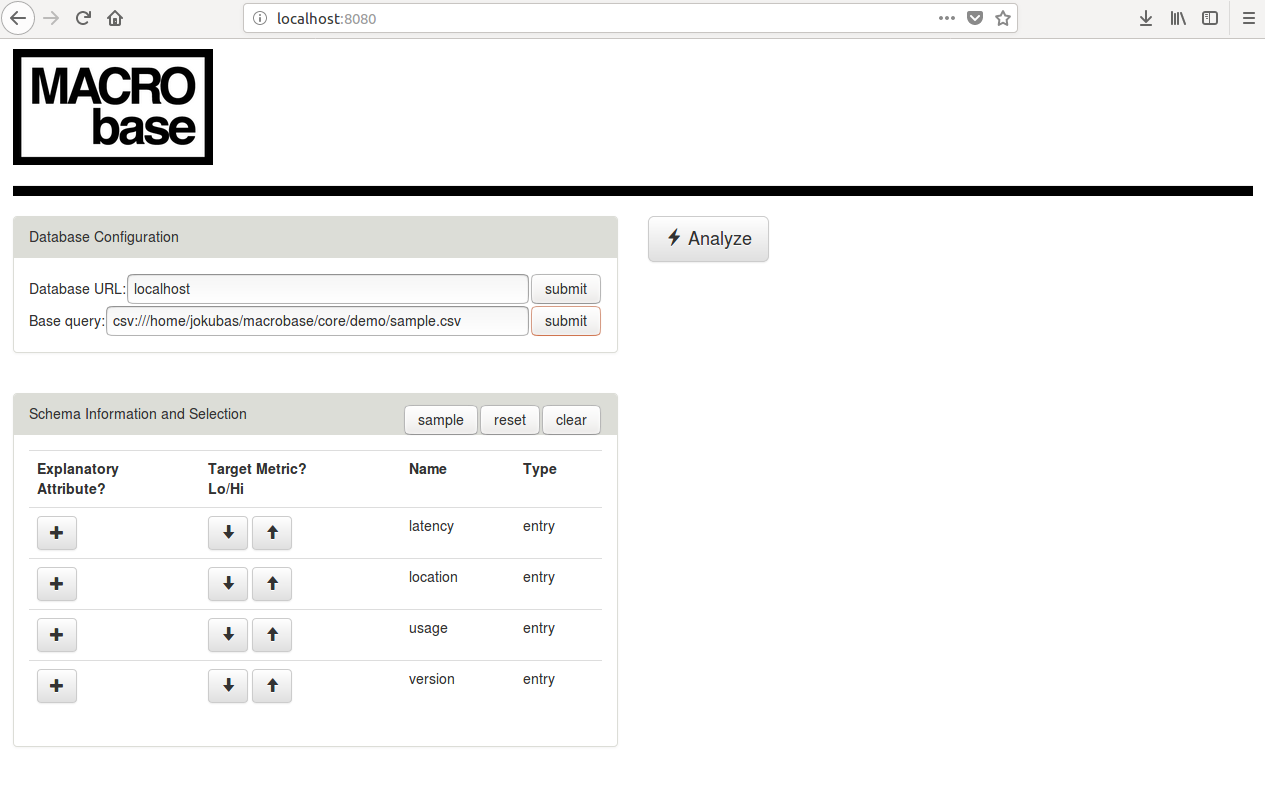
\includegraphics[scale=0.33]{img/gui}
    \caption{„MacroBase GUI“ pagrindinis langas}
    \label{img:gui}
\end{figure}
\begin{figure}[H]
    \centering
    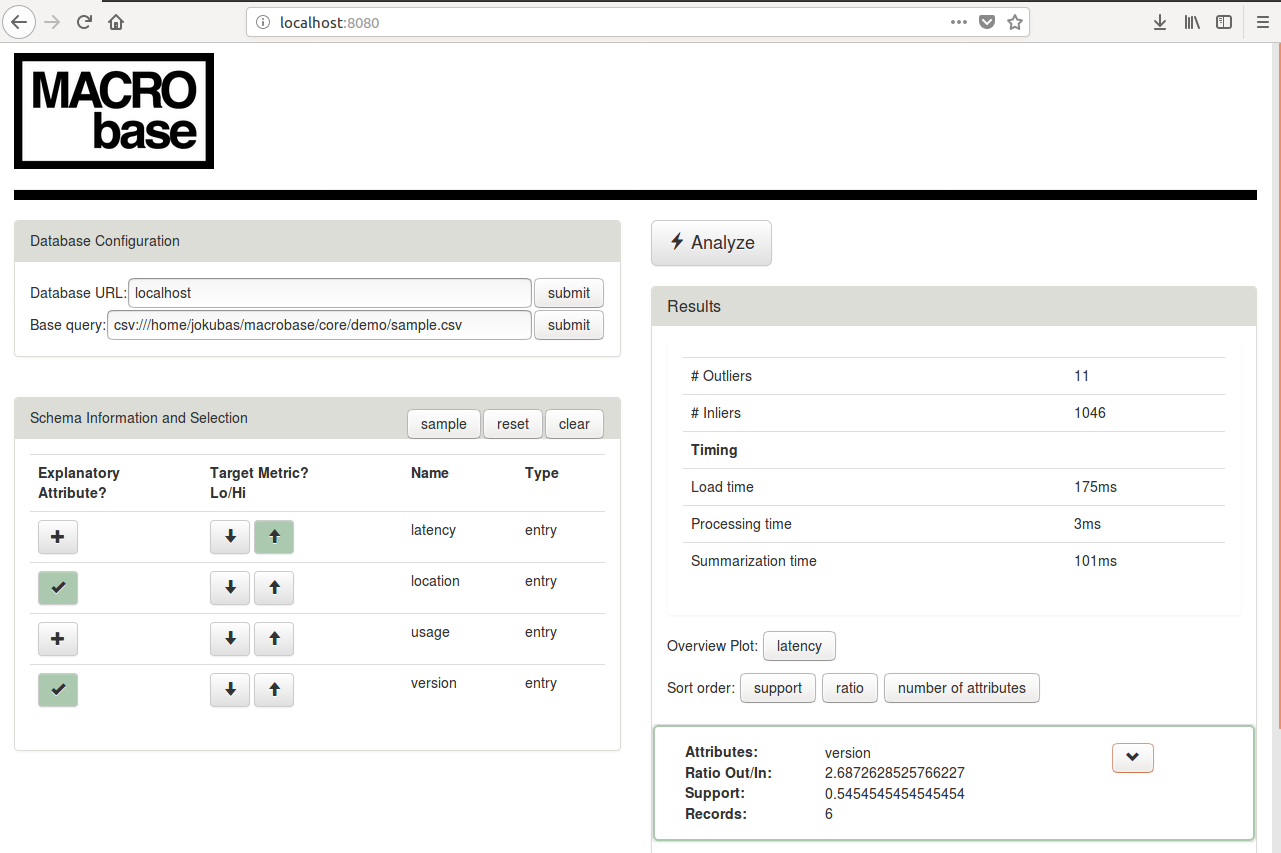
\includegraphics[scale=0.33]{img/gui2}
    \caption{„MacroBase GUI“ pagrindinis langas su analizės rezultatais}
    \label{img:gui2}
\end{figure}

\end{document}
